\PassOptionsToPackage{unicode=true}{hyperref} % options for packages loaded elsewhere
\PassOptionsToPackage{hyphens}{url}
%
\documentclass[english,man]{apa6}
\usepackage{lmodern}
\usepackage{amssymb,amsmath}
\usepackage{ifxetex,ifluatex}
\usepackage{fixltx2e} % provides \textsubscript
\ifnum 0\ifxetex 1\fi\ifluatex 1\fi=0 % if pdftex
  \usepackage[T1]{fontenc}
  \usepackage[utf8]{inputenc}
  \usepackage{textcomp} % provides euro and other symbols
\else % if luatex or xelatex
  \usepackage{unicode-math}
  \defaultfontfeatures{Ligatures=TeX,Scale=MatchLowercase}
\fi
% use upquote if available, for straight quotes in verbatim environments
\IfFileExists{upquote.sty}{\usepackage{upquote}}{}
% use microtype if available
\IfFileExists{microtype.sty}{%
\usepackage[]{microtype}
\UseMicrotypeSet[protrusion]{basicmath} % disable protrusion for tt fonts
}{}
\IfFileExists{parskip.sty}{%
\usepackage{parskip}
}{% else
\setlength{\parindent}{0pt}
\setlength{\parskip}{6pt plus 2pt minus 1pt}
}
\usepackage{hyperref}
\hypersetup{
            pdftitle={Development of infants' preference for speech: Meta-analytic evidence},
            pdfkeywords={Meta-analysis, Infants, Speech preference, Conspecific detection, Developmental tuning},
            pdfborder={0 0 0},
            breaklinks=true}
\urlstyle{same}  % don't use monospace font for urls
\usepackage{graphicx,grffile}
\makeatletter
\def\maxwidth{\ifdim\Gin@nat@width>\linewidth\linewidth\else\Gin@nat@width\fi}
\def\maxheight{\ifdim\Gin@nat@height>\textheight\textheight\else\Gin@nat@height\fi}
\makeatother
% Scale images if necessary, so that they will not overflow the page
% margins by default, and it is still possible to overwrite the defaults
% using explicit options in \includegraphics[width, height, ...]{}
\setkeys{Gin}{width=\maxwidth,height=\maxheight,keepaspectratio}
\setlength{\emergencystretch}{3em}  % prevent overfull lines
\providecommand{\tightlist}{%
  \setlength{\itemsep}{0pt}\setlength{\parskip}{0pt}}
\setcounter{secnumdepth}{0}

% set default figure placement to htbp
\makeatletter
\def\fps@figure{htbp}
\makeatother

% Manuscript styling
\usepackage{upgreek}
\captionsetup{font=singlespacing,justification=justified}

% Table formatting
\usepackage{longtable}
\usepackage{lscape}
% \usepackage[counterclockwise]{rotating}   % Landscape page setup for large tables
\usepackage{multirow}		% Table styling
\usepackage{tabularx}		% Control Column width
\usepackage[flushleft]{threeparttable}	% Allows for three part tables with a specified notes section
\usepackage{threeparttablex}            % Lets threeparttable work with longtable

% Create new environments so endfloat can handle them
% \newenvironment{ltable}
%   {\begin{landscape}\begin{center}\begin{threeparttable}}
%   {\end{threeparttable}\end{center}\end{landscape}}
\newenvironment{lltable}{\begin{landscape}\begin{center}\begin{ThreePartTable}}{\end{ThreePartTable}\end{center}\end{landscape}}

% Enables adjusting longtable caption width to table width
% Solution found at http://golatex.de/longtable-mit-caption-so-breit-wie-die-tabelle-t15767.html
\makeatletter
\newcommand\LastLTentrywidth{1em}
\newlength\longtablewidth
\setlength{\longtablewidth}{1in}
\newcommand{\getlongtablewidth}{\begingroup \ifcsname LT@\roman{LT@tables}\endcsname \global\longtablewidth=0pt \renewcommand{\LT@entry}[2]{\global\advance\longtablewidth by ##2\relax\gdef\LastLTentrywidth{##2}}\@nameuse{LT@\roman{LT@tables}} \fi \endgroup}

% \setlength{\parindent}{0.5in}
% \setlength{\parskip}{0pt plus 0pt minus 0pt}

% \usepackage{etoolbox}
\makeatletter
\patchcmd{\HyOrg@maketitle}
  {\section{\normalfont\normalsize\abstractname}}
  {\section*{\normalfont\normalsize\abstractname}}
  {}{\typeout{Failed to patch abstract.}}
\makeatother
\shorttitle{Preference for speech sounds in infancy}
\author{Cécile Issard\textsuperscript{1}, Sho Tsuji\textsuperscript{2}, \& Alejandrina Cristia\textsuperscript{1}}
\affiliation{
\vspace{0.5cm}
\textsuperscript{1} Laboratoire de Sciences Cognitives et Psycholinguistique, Ecole Normale Supérieure, Département d'Études Cognitives\\\textsuperscript{2} International Research Center for Neurointelligence, The University of Tokyo}
\authornote{This work was supported by an Agence Nationale de la Recherche grant to A.C. (ANR-17-CE28-0007 LangAge, ANR-16-DATA-0004 ACLEW, ANR-14-CE30-0003 MechELex, ANR-17-EURE-0017); and the J. S. McDonnell Foundation Understanding Human Cognition Scholar Award to A.C.

The authors declare no conflict of interest. Funding sources did not take part in study design, data collection or analysis.

Our data is fully available in the corresponding OSF repository: http://tidy.ws/bqjc4U

We thank Chiara Santolin, Martin Zettersten, Jenny Saffran, Christina Vanden Bosch Der Nederlanden, and Athena Vouloumanos for contributing unpublished data.


Correspondence concerning this article should be addressed to Cécile Issard, Laboratoire de Sciences Cognitives et Psycholinguistique, Département d'Études Cognitives, Ecole Normale Supérieure, 29 rue d'Ulm, 75005 Paris, France. E-mail: cecile.issard@gmail.com}
\keywords{Meta-analysis, Infants, Speech preference, Conspecific detection, Developmental tuning\newline\indent Word count: }
\DeclareDelayedFloatFlavor{ThreePartTable}{table}
\DeclareDelayedFloatFlavor{lltable}{table}
\DeclareDelayedFloatFlavor*{longtable}{table}
\makeatletter
\renewcommand{\efloat@iwrite}[1]{\immediate\expandafter\protected@write\csname efloat@post#1\endcsname{}}
\makeatother
\usepackage{csquotes}
\ifnum 0\ifxetex 1\fi\ifluatex 1\fi=0 % if pdftex
  \usepackage[shorthands=off,main=english]{babel}
\else
  % load polyglossia as late as possible as it *could* call bidi if RTL lang (e.g. Hebrew or Arabic)
  \usepackage{polyglossia}
  \setmainlanguage[]{english}
\fi

\title{Development of infants' preference for speech: Meta-analytic evidence}

\date{}

\abstract{
Numerous species, such as primates and songbirds, use vocal communication to build social interactions. Accordingly, they must be able to pay attention to their conspecifics' vocalizations. Previous experimental studies suggested that in humans, these skills develop from early infancy, with infants showing a preference for speech over other sounds, but the mechanism underlying the preference remains unclear, with some results pointing to a preference for (a) familiar sounds; (b) vocal sounds; or (c) natural sounds more generally, with potential changes over development. To shed light on whether some of these mechanisms may be at play, we conducted a meta-analysis of experiments testing speech preference in infants. Synthesizing data from 775 infants across 38 experiments, we found that infants reliably preferred speech over other sounds, but this preference was not significantly moderated by familiarity, vocal quality, or naturalness of the competitor. Also, we found no effect of age: infants showed the same strength of preference throughout the first year of life. Speech therefore appears to be preferred from birth, even to other natural or vocal sounds. These results nuance current views of the development of speech perception, and call for further investigation of the phenomenon.
}

\begin{document}
\maketitle

\hypertarget{significance}{%
\section{Significance}\label{significance}}

\begin{itemize}
\tightlist
\item
  Infants reliably prefer natural speech over other types of sounds, from birth to the end of the first year of life
\item
  Speech is preferred over both artificial and other natural sounds
\item
  Speech is preferred over both non-vocal and other vocal sounds
\item
  The difference between whether infants are familiar or not with the language used was not significant
\end{itemize}

\hypertarget{introduction}{%
\section{Introduction}\label{introduction}}

In gregarious species, the ability of individuals to orient their attention towards conspecifics' vocalizations is crucial for social interactions and communication. Correspondingly, numerous results have demonstrated processing advantages for conspecific vocalizations in a wide variety of species, including primates and birds (Poremba, Bigelow, \& Rossi, 2013). Previous work has suggested that in humans, communication skills develop from early infancy, manifesting in an early preference for speech over other types of sound (Ecklund-Flores \& Turkewitz, 1996; Vouloumanos, Hauser, Werker, \& Martin, 2010; Vouloumanos \& Werker, 2007). This preference may emerge through a variety of simpler mechanisms, saliently including a preference for familiar over unfamiliar sounds, natural over artificial sounds, and vocal over non-vocal sounds (Figure \ref{fig:venn}). Here, we synthesize the available empirical data on infants' preferences for speech over non-speech sounds to assess the size of this effect, and the explanatory role of these mechanisms.

\begin{figure}
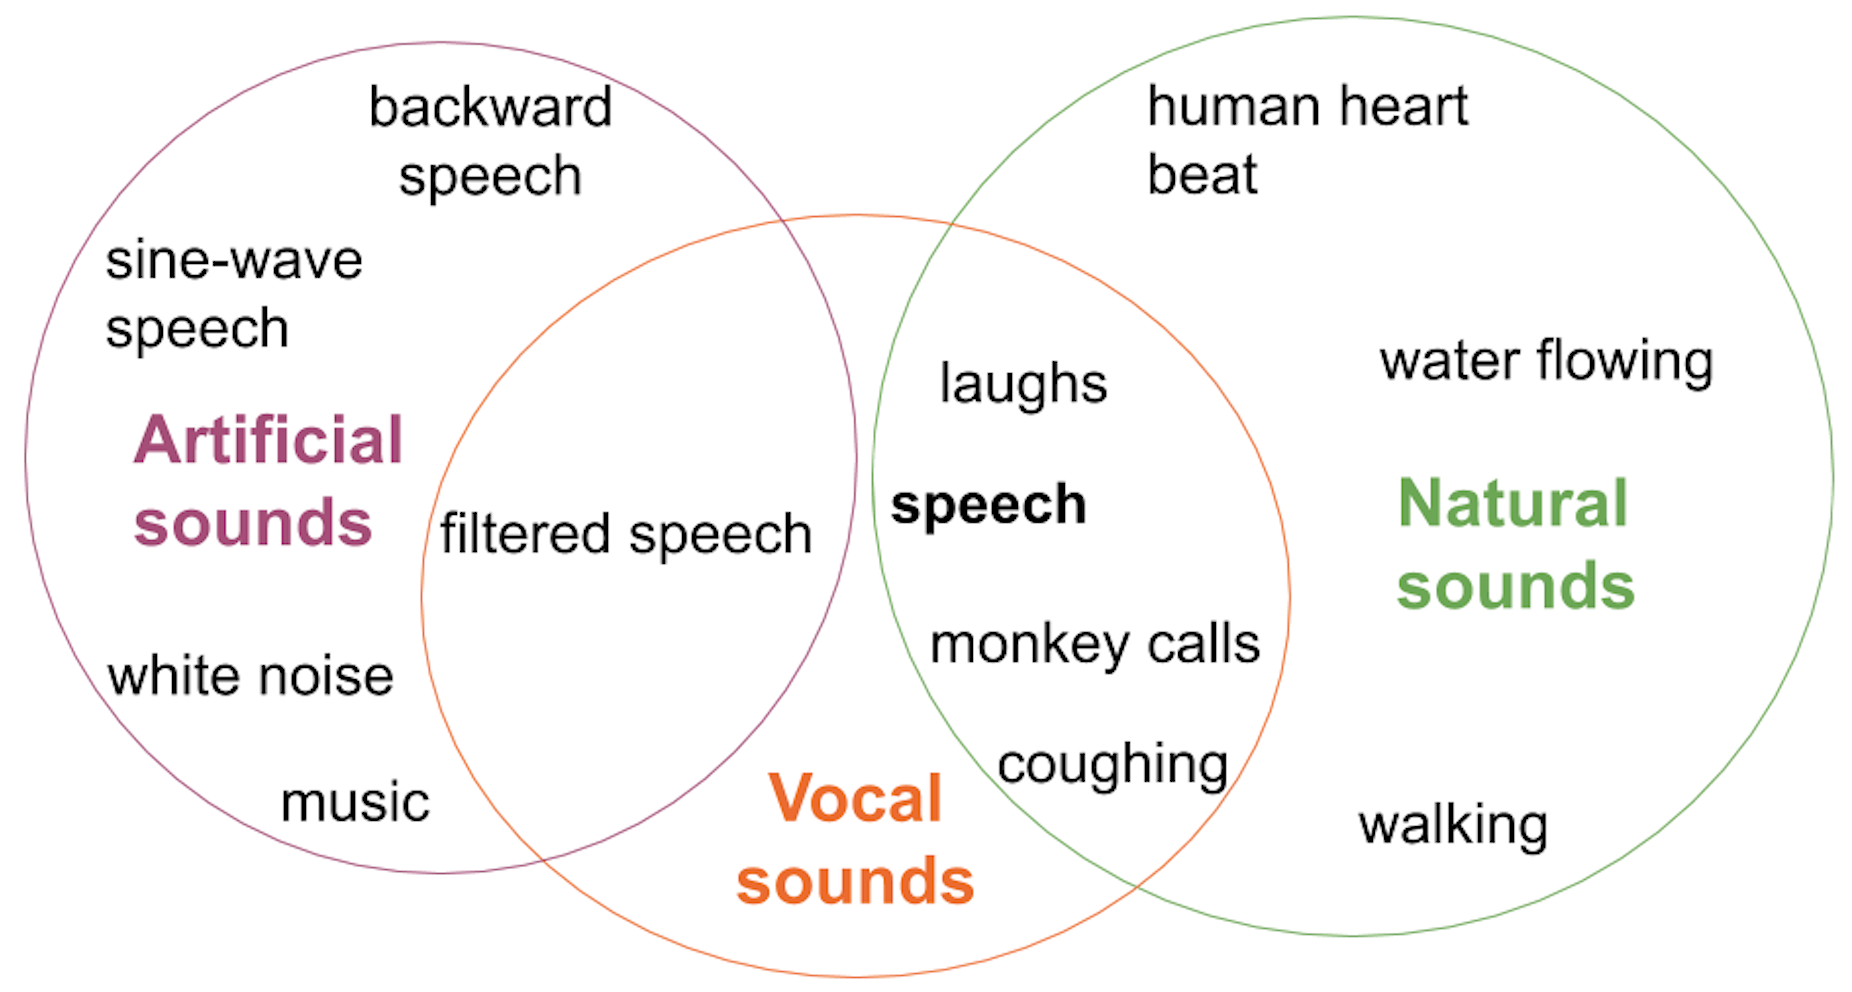
\includegraphics[width=6.17in]{figures_intro/Venn} \caption{Speech is a natural, vocal sound.}\label{fig:venn}
\end{figure}

One mechanism could involve familiarity: Perhaps infants prefer speech to other sounds because speech is a frequent sound in their experience. Newborns prefer their native speech to prosodically distinct foreign speech (e.g., Mehler et al., 1988; Moon, Cooper, \& Fifer, 1993), which supports a preference for sound patterns heard frequently in the womb. If this mechanism is at play in speech preference, infants should show a stronger preference for speech over other sounds when tested in their native language, and a weaker preference when tested with a foreign language.

A second mechanism could involve a preference for natural over artificial sounds. Natural sounds are those produced by biological systems, such as heart beats, step sounds, or animal vocalizations, and environmental/geophysical sounds, such as wind, rain, or the sound of a river. Natural sounds are processed more efficiently by the auditory system, from the cochlea (Smith \& Lewicki, 2006) to the auditory cortex (see Mizrahi, Shalev, \& Nelken, 2014 for a review). If this mechanism (partially) explains speech preferences, then we should observe that the preference for speech over artificial competitors is stronger than the preference observed when contrasting speech against another natural sounds.

A third mechanism would rely on a preference for vocal sounds. It is possible that infants initially form a broad category of vocal sounds, including the vocalizations of other species that use oral communication (e.g.~other primates and birds), these vocalizations potentially sharing some important acoustical properties with speech. Vocal sounds have acoustic signatures, since they are characterized by modulations introduced by the vocal tract, with harmonically related energy peaks. If this mechanism explains at least partially speech preferences, the preference for speech over non-vocal competitors would be stronger than the preference observed when contrasting speech against other vocal sounds.

Development may affect the preference for speech in various ways. For example, whereas newborns do not prefer speech over monkey calls, there is some evidence that three-month-olds do (Vouloumanos et al., 2010). Both maturation and experience could affect the extent to which naturalness, familiarity, and vocal quality affect infants' preferences as a function of age. In this case, the capacity to preferentially respond to speech as compared to other sounds is thought to come from a dynamic process of narrowing the perceptual category from natural or vocal sounds to speech specifically.

\hypertarget{a-meta-analytic-approach}{%
\subsection{A meta-analytic approach}\label{a-meta-analytic-approach}}

In sum, previous results on infants' preference for speech are broadly compatible with a preference for natural over artificial, vocal over non-vocal, and/or familiar over unfamiliar sounds, potentially interacting with infants' age. In this paper, we seek to directly test these potential mechanisms by employing a meta-analytic approach.

A meta-analysis can integrate data from experiments that vary in their methodology, as well as test the effect of factors of theoretical importance, by redescribing the stimuli used as a function of those factors. For instance, a study measuring preference for native speech over native backward speech provides data on a natural versus artificial contrast, as well as a vocal versus non-vocal contrast.

Also, we can draw a developmental timeline across the age range covered by the literature, beyond age groups tested within papers. This is particularly useful in developmental psychology, that rely on age-related phenomenons that need to be tested statistically (Gelman \& Stern, 2006). Meta-analysis offer a powerful statistical approach to directly test for interactions with age across the whole age-range covered by the literature. To give an example from a previous developmental meta-analysis, it had been proposed that infants' preference for novel or familiar items related to infants' age such that, all things equal, younger infants showed familiarity preferences whereas older infants exhibited novelty preferences (Hunter \& Ames, 1988). However, stable familiarity preferences across the first two years have been found for word segmentation in natural speech (Bergmann \& Cristia, 2016); and a stable novelty effect ensues for artificial grammars implemented in synthesized speech, whereas those implemented in natural speech led to stable familiarity preferences (Black \& Bergmann, 2017). Meta-analyses are therefore important to statistically and systematically test the theoretical predictions proposed in qualitative reviews, and refine current readings of a literature.

Single experiments tell us about what a specific group of participants, presented with a specific set of stimuli, in a specific point in time has done. Meta-analyses are the following step because they provide a principled statistical approach to integrate those individual and specific results into a larger picture. By aggregating the numerous individual studies of a literature, meta-analyses gain statistical power. As a result, meta-analyses can reveal small effects that are difficult to show in individual experiments. By integrating data across different laboratories, they provide evidence for the generalizability of effects, and facilitate comparisons between experimental results.

Finally, meta-analyses offer tools to detect publication bias in the literature. By aggregating all the available evidence for a phenomenon, we can see if the distribution of effect sizes has an unexpected shape, typically with an excess of positive results due to the difficulty to publish null or negative results. We can further integrate this information, and derive a new estimate of the overall effect size.

\hypertarget{the-present-study}{%
\subsection{The present study}\label{the-present-study}}

Although we were primarily motivated by a theoretical quest, we know meta-analyses provide a unique vantage point on a body of work as a whole. We therefore first check for how strong infants' preference for speech over other types of sounds is according to the public body of literature. We additionally assess this body of data for evidence of publication bias.

We then turn to our key interest, namely shedding light on the potential mechanisms underlying infants' speech preferences. Meta-regressions assess whether the proposed mechanisms of familiarity, naturalness, and vocal quality drive this preference, and how the preference develops over the first year of life. Assuming all three mechanisms are at play, and further assuming that the definition of the preferred stimulus narrows with age, we predicted that infants will show (see Figure \ref{fig:hyp}):

\begin{enumerate}
\def\labelenumi{\arabic{enumi}.}
\tightlist
\item
  a greater preference for native speech over non-speech as a function of age, but a smaller preference for foreign speech over non-speech with age;
\item
  a greater preference for speech over other natural sounds as a function of age, but a preference for speech over artificial sounds that is stable over development;
\item
  a greater preference for speech over other vocal sounds as a function of age, but a stable preference for speech over non-vocal sounds over development.
\end{enumerate}

\begin{figure}
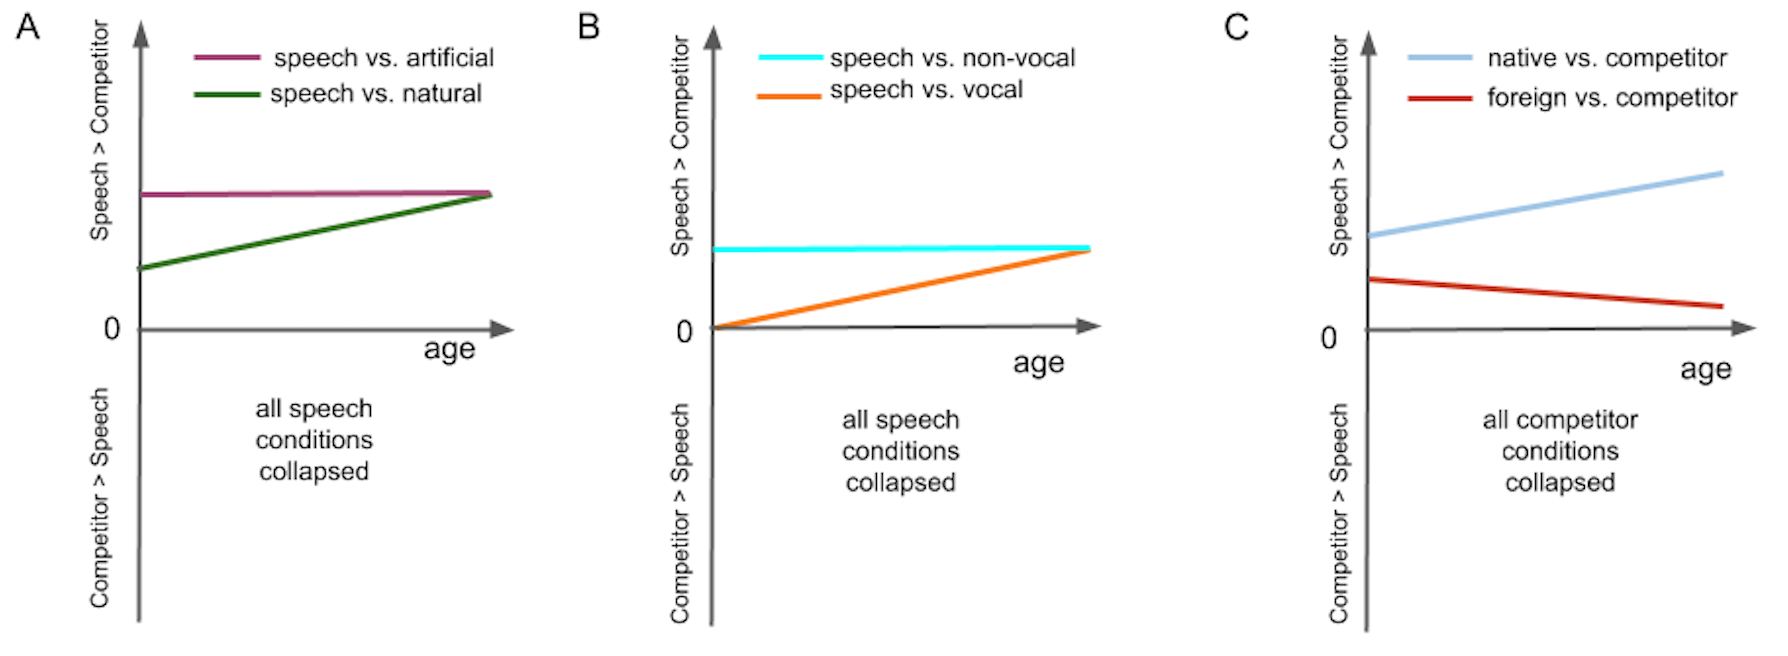
\includegraphics[width=3.2in]{figures_intro/hypotheses} \caption{Hypothesized pattern of preference: the x axis shows age, the y axis represents the effect size derived from the contrast between a speech condition and a competitor condition (preference for speech over the competitor is plotted up; the lower quadrants are empty because we do not predict a preference for the competitor over speech). A: Speech contrasted to natural (green) or artificial (purple) competitors. B: Speech contrasted to vocal (orange) or non-vocal (cyan) competitors. C: Collapsing across competitors, separating speech in a foreign language (red); speech in the native language (blue).}\label{fig:hyp}
\end{figure}

\hypertarget{methods}{%
\section{Methods}\label{methods}}

This meta-analysis was carried out following PRISMA recommendations (Moher, Liberati, Tetzlaff, Altman, \& Group, 2009). In addition, we provide information on all steps (including PRISMA checklist, data, and code) for full transparency and accountability via online supplementary materials; \url{https://osf.io/4stz9/?view_only=d0696591ebf34bfc8430f848cd945ca8}.

\hypertarget{literature-search}{%
\subsection{Literature search}\label{literature-search}}

We composed the initial list of papers with suggestions by experts (authors of this work); one google scholar search (\emph{(\enquote{speech preference} OR \enquote{own-species vocalization}) AND infant - \enquote{infant-directed}}), the same search in PubMed and PsycInfo (last searched on 2019-09-24); and a google alert. We also inspected the reference lists of all included papers. Finally, we emailed a major mailing list to ask for missing data. We received two replies, one of which revealed a formerly undiscovered published study, and communicated unpublished data (Santolin, Zettersten, \& Saffran, 2020).

\hypertarget{inclusion-criteria}{%
\subsection{Inclusion criteria}\label{inclusion-criteria}}

After a first screening based on titles and abstracts using more liberal inclusion criteria, we decided on final inclusion based on full paper reading. We included experiments that tested human infants from birth to one year of age, and contrasted speech sounds with any other type of sound, measuring behavioral preferences to the sounds (e.g., looking times). If a paper reported results from neurotypical and at-risk infants, we included only the data from the neurotypical group.

Given our key interest in the preference for speech over other sounds, we excluded studies that contrasted two different speech sounds (e.g., foreign vs.~native language, or adult vs.~child-directed speech, or mother vs.~stranger's voice); or two different non-speech sounds (e.g., backward speech vs.~animal vocalizations). In addition, we excluded experiments where the contrast presented to the infants could not be coded according to our three mechanistic explanations. This meant the exclusion of experiments where speech was presented in the mother's voice (which thus confounds between speech and individual voice recognition for our familiarity factor). Finally, we excluded neuroimaging experiments to avoid mixing results from different brain regions with different response profiles. We included published (i.e., journal articles) as well as unpublished works (i.e., doctoral dissertations) as long as sufficient information was provided.

A PRISMA flow chart summarizes the literature review and selection process (Figure \ref{fig:prisma}). The full list of the papers that were inspected together final inclusion decisions are available in a decision spreadsheet (see the online supplementary materials; \url{https://osf.io/4stz9/?view_only=d0696591ebf34bfc8430f848cd945ca8}).

\begin{figure}
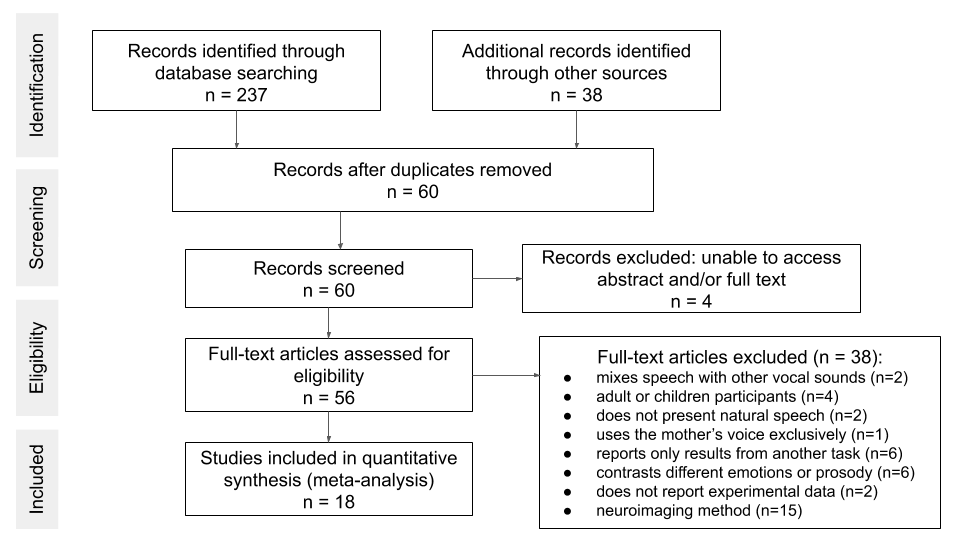
\includegraphics[width=3.2in]{figures_intro/PRISMA} \caption{PRISMA flowchart summarizing the literature review and selection process.}\label{fig:prisma}
\end{figure}

\hypertarget{coding}{%
\subsection{Coding}\label{coding}}

Data were coded by the first author. In addition, 20\% of the papers were randomly selected to be coded by the last author independently, with disagreements resolved by discussion. There were 10 disagreements out of a total of 260 fields filled in, and they were indicative of the coders not following the codebook, which led to a revision of all data in four variables.

The critical variables for our purpose are key stimuli characteristics, infant age, and testing method (central fixation, high amplitude sucking, head-turn preference procedure). As for key stimuli characteristics, we coded familiarity, naturalness, and vocal quality, as follows.

For \textbf{familiarity}, we considered the language in which the speech sounds were recorded (native or foreign).

For \textbf{naturalness}, the competitor sound was coded as natural if it was produced by a biological organism without any further acoustic manipulation. Natural competitors included animal calls, environmental sounds (e.g.~wind or water sounds), heartbeat, bird song, non-speech vocalizations (e.g.~laughters or coughs). If the authors applied acoustic manipulations, the competitor was coded as artificial. Artificial competitors included sine-wave speech, filtered speech\footnote{In the case of filtered speech, the modulations introduced by the vocal tract are still present at the retained frequencies, and formant transitions are consistent with vocal production constraints. For this reason, filtered speech can be considered as vocal but not natural. Because the womb acts as a low-pass filter, newborn infants are familiar with low-pass filtered speech, but this familiarity fades after birth.}, white noise, instrumental music, and speech with altered rhythmic structure. The only exception was for newborn experiments presenting low-pass filtered speech mimicking the filtering applied by the womb. Given the recency of the intra-uterine environement to newborns (about 2 days), we coded these as natural.

For \textbf{vocal quality}, the competitor sound was considered as vocal if it was produced by an animal vocal tract (human or not), either original or modified. Vocal competitors included non-speech vocalizations, animal calls, bird songs, and filtered speech. Non-vocal competitors included backward speech (that has abrupt closures that cannot be produced by the vocal tract), white-noise, environmental sounds, instrumental music, heartbeat, and sine-wave speech (that lacks the harmonic structure introduced by the natural resonance of the vocal tract).

We coded all the statistical information reported in the included papers. If reported, we coded the mean score and the standard deviation for speech, and the other sound separately. When infant-level data was provided, we recomputed the respective mean scores and standard deviations based on the reported individual scores. If reported, we also coded the t-statistic between the two sound conditions, or an F-statistic provided this was a two-way comparison. If effect sizes were directly reported as a Cohen's d or a Hedges' g, we also coded this.

\hypertarget{effect-sizes}{%
\subsection{Effect sizes}\label{effect-sizes}}

Once the data were coded, we extracted effect sizes, along with their respective variance. Effect sizes were standardized differences (Cohen's d) between response to speech vs.~the competitor.
If effect sizes were not directly reported in the papers, we computed them using the respective means and SDs (Lipsey \& Wilson, 2001), or a t- or F-statistic (Dunlap, Cortina, Vaslow, \& Burke, 1996). As our effect sizes came from within-subject comparisons (e.g., looking time of the same infant during speech and during monkey calls), we needed to take into account the correlation between the two measurements in effect sizes and effect size variances computations. We computed this correlation based on the t-statistic, the respective means and SDs (Lipsey \& Wilson, 2001) if they were all reported; or imputed this correlation randomly if not. We finally calculated the variance of each effect size (Lipsey \& Wilson, 2001). Cohen's d were transformed to Hedges' g by multiplying d by a correction for small sample sizes based on the degree of freedom (Borenstein, Hedges, Higgins, \& Rothstein, 2011).

We did not center age because our hypotheses included a developmental progression from birth to the end of the first year of life. We were therefore interested in the intercept at age 0 (i.e., birth).

Analyses use the R (R Core Team, 2018) package Robumeta (Hedges, Tipton, \& Johnson, 2010), which allows us to fit meta-analytic regressions that take into account the correlated structure of the data, when repeated measures are obtained from the same infant groups within papers.

\hypertarget{results}{%
\section{Results}\label{results}}

\hypertarget{database-description}{%
\subsection{Database description}\label{database-description}}

We found a total of 18 publications (labeled with an asterisk in the reference list) reporting 38 experiments, for a total of \texttt{sum(temp\$n)} infants, and 54 (not mutually independent) effect sizes, see Figure \ref{fig:forest}. 15 papers have been submitted to or published in peer-reviewed journals (Colombo \& Bundy, 1981; Cooper \& Aslin, 1994; Curtin \& Vouloumanos, 2013; Ecklund-Flores \& Turkewitz, 1996; Santolin, Russo, Calignano, Saffran, \& Valenza, 2019; Segal \& Kishon-Rabin, 2011; Shultz \& Vouloumanos, 2010; Sorcinelli, Ference, Curtin, \& Vouloumanos, 2019; Spence \& DeCasper, 1987; Vanden Bosch der Nederlanden \& Vouloumanos, 2020; Vouloumanos \& Curtin, 2014; Vouloumanos, Druhen, Hauser, \& Huizink, 2009; Vouloumanos et al., 2010, 2010; Vouloumanos \& Werker, 2004, 2007; Yamashiro, Curtin, \& Vouloumanos, 2019). The remaining 1 publication contributing 8 effect size was a thesis (Ference, 2018). 6 more effect sizes were contributed by authors of unpublished work (Santolin et al., 2020).

Experiments tended to have small sample sizes, with a median N of 16 children (Range = {[}60, 4{]}, M = 19.83, Total: 775), which is close to the field standard (Bergmann et al., 2018), but much lower than current recommendations (Oakes, 2017). Infants ranged from 0 to 12 months (1.50 to 380.50 days), although the majority were under 6 months of age (63.16\% of the experiments). Individual samples comprised 46\% of female participants on average. Infants were native of 6 different languages across the whole database (English, French, Russian, Yiddish, Hebrew, Italian).
Experiments were performed in 10 different laboratories from 4 different countries (United States, Canada, Israel, Italy). 3 experimental methods were used: 30 experiments used Central Fixation (CF) (also called sequential looking preference procedure) (Colombo \& Bundy, 1981; Cooper \& Aslin, 1994; Curtin \& Vouloumanos, 2013; Ference, 2018; Santolin et al., 2019, 2020; Segal \& Kishon-Rabin, 2011; Shultz \& Vouloumanos, 2010; Sorcinelli et al., 2019; Vanden Bosch der Nederlanden \& Vouloumanos, 2020; Vouloumanos \& Curtin, 2014; Vouloumanos et al., 2009, 2010; Vouloumanos \& Werker, 2004; Yamashiro et al., 2019); 3 used High-Amplitude Sucking (HAS) (Spence \& DeCasper, 1987; Vouloumanos et al., 2010; Vouloumanos \& Werker, 2007); and 5 used Head-turn Preference Procedure (HPP) (Ecklund-Flores \& Turkewitz, 1996). Trial length was fixed in 8 experiments, and infant-controlled in 29 experiments.

Speech sounds were spoken by a female in 36 out of 38 experiments, with an infant-directed prosody in 21 out of the 38 experiments. Speech was presented in isolated segments (i.e.~words or syllables) in 5 experiments, and full sentences or passages in 19 experiments. Speech stimuli were recorded in the infant native language in 63.16\% of the experiments. Strikingly, experiments using the infants' native language tested infants from 0 to 12 months of age, whereas experiments using a foreign language only tested infants from 3 to 9 months of age (see Figure \ref{fig:lang}).
The competitor sound was vocal in 47.37\% of the experiments. The competitor sound was natural 47.37\% of the experiments.
The stimuli characteristics are summarized on Supplementary Figures S\ref{fig:stimuli} and \ref{fig:competitors}.

\begin{figure}
\centering
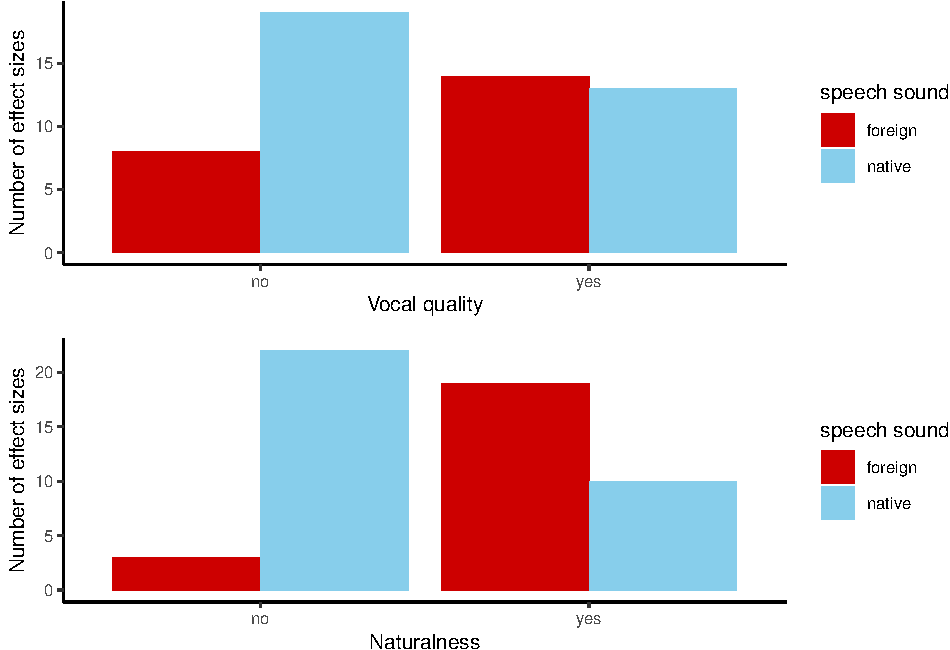
\includegraphics{MA_speech_pref_files/figure-latex/stimuli-1.pdf}
\caption{\label{fig:stimuli}Histograms of the number of effect sizes for each language and moderator status.}
\end{figure}

\begin{figure}
\centering
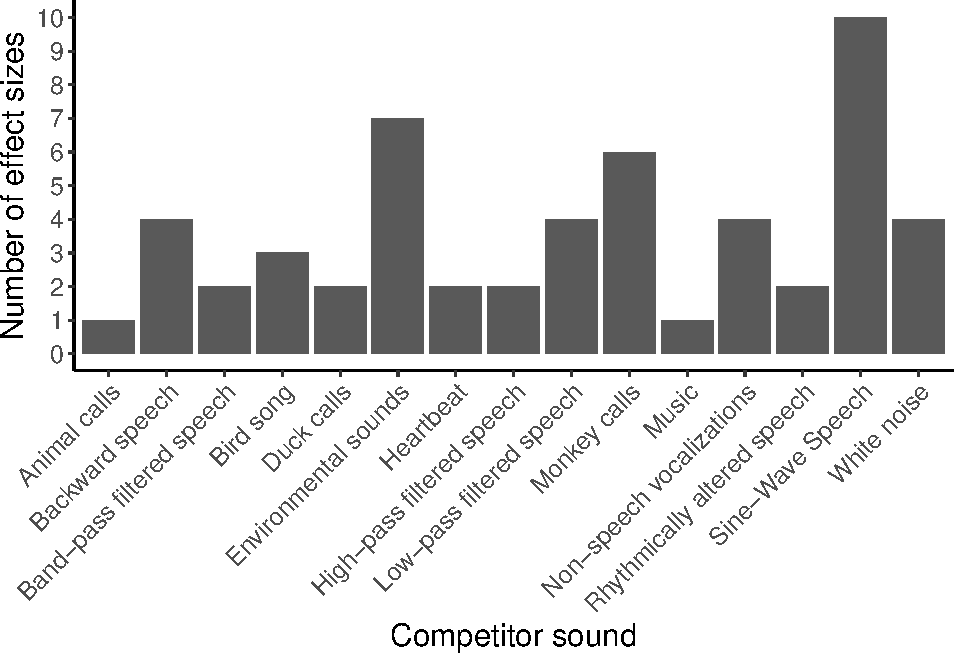
\includegraphics{MA_speech_pref_files/figure-latex/competitors-1.pdf}
\caption{\label{fig:competitors}Histogram of the number of effect sizes for each competitor.}
\end{figure}

\hypertarget{average-effect-size}{%
\subsection{Average effect size}\label{average-effect-size}}

\begin{figure}
\centering
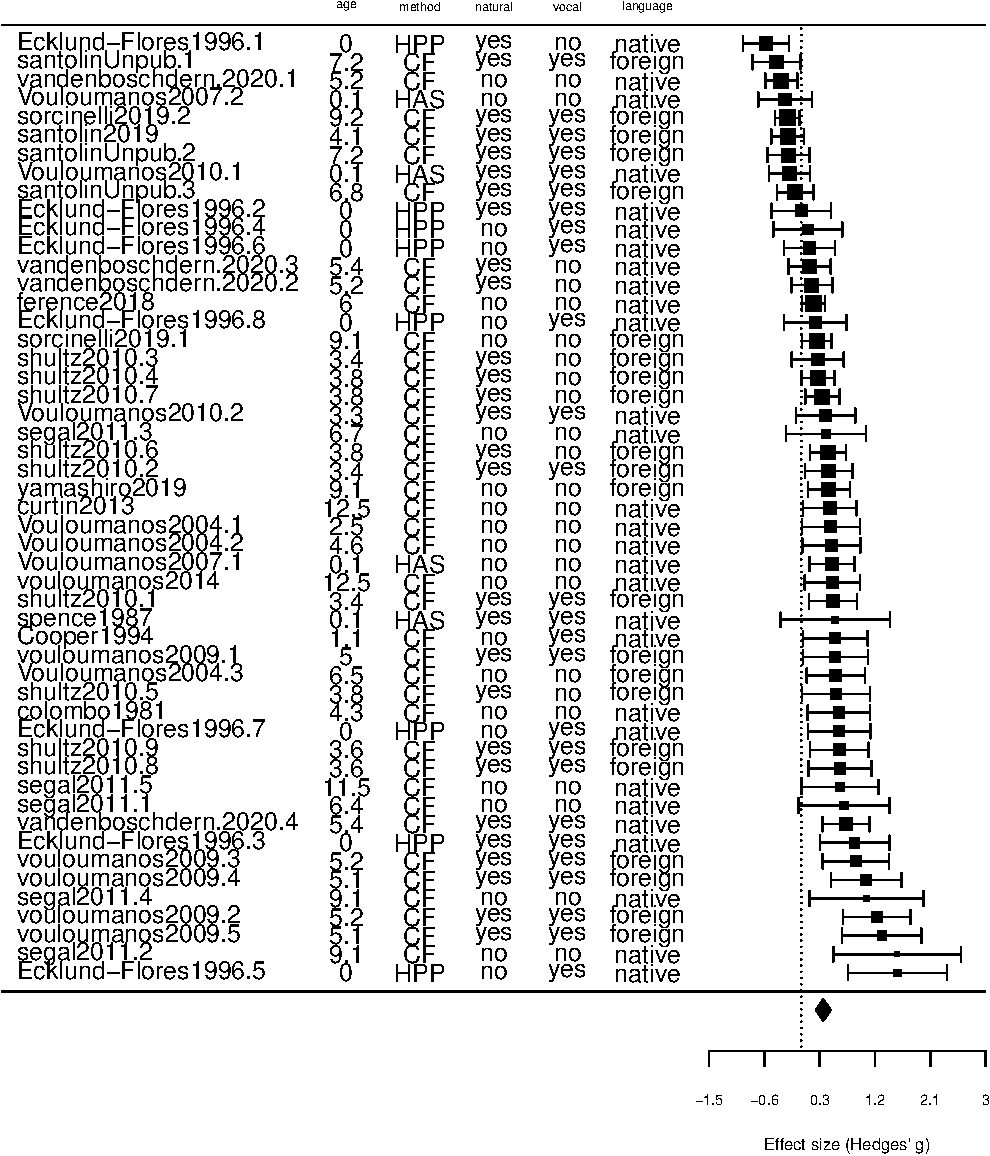
\includegraphics{MA_speech_pref_files/figure-latex/forest-1.pdf}
\caption{\label{fig:forest}Forest plot of effect sizes available in the literature, along with their respective moderator status. The average effect size is plotted on the bottom line.}
\end{figure}

We integrated all effect sizes in a meta-analytic regression without any moderator, and found an average effect size g of 0.35 (SE = 0.06, CI = {[}0.22 , 0.48{]}) (Table 1, and Figure \ref{fig:forest}, diamond), corresponding to a medium effect size.
Heterogeneity among effect sizes was estimated at \(\tau^2\) = 0.13 (I\textsuperscript{2} = 77.08\%), which was significant (Q = 202.15, p \textless{} 0.01) despite the removal of outliers before running the model. This strongly suggest differences across experiments, and invites analyses using moderators.

\begin{table}[tbp]

\begin{center}
\begin{threeparttable}

\caption{\label{tab:Table1}Statistical results of meta-regression without any moderator.}

\begin{tabular}{lcccc}
\toprule
 & estimate & SE & t & confidence interval\\
\midrule
average effect size & 0.35 & 0.06 & 5.52 & 0.22 - 0.48\\
\bottomrule
\end{tabular}

\end{threeparttable}
\end{center}

\end{table}

\hypertarget{publication-bias}{%
\subsection{Publication bias}\label{publication-bias}}

\begin{figure}
\centering
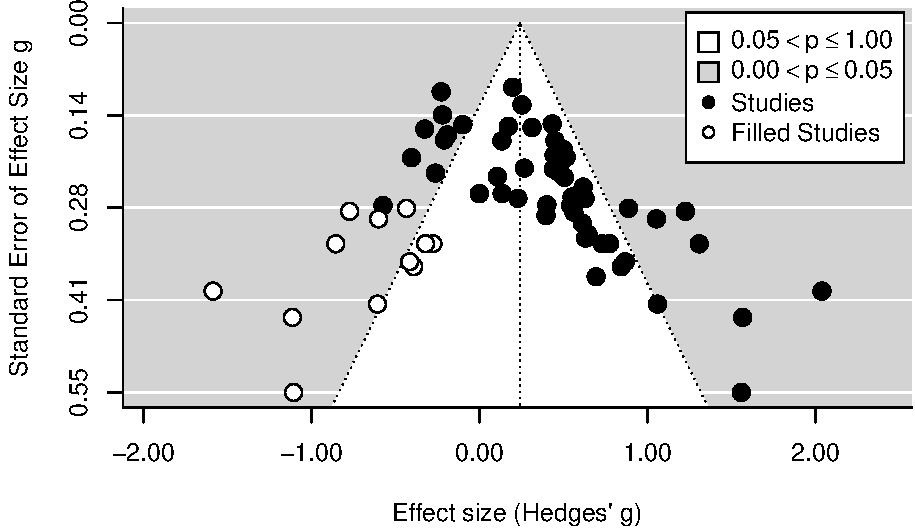
\includegraphics{MA_speech_pref_files/figure-latex/bias-1.pdf}
\caption{\label{fig:bias}Funnel plot of effect sizes and their respective standard errors. Black dots: effect sizes observed in the literature. White dots: missing effect sizes, suggestive of a publication bias\(^2\). Vertical line: average effect size after filling the missing effect sizes.}
\end{figure}

We checked for the presence of a potential publication bias in the body of literature by studying the relationship between standard errors of effect sizes as a function of Hedges' g (see funnel plot in Figure \ref{fig:bias})\footnote{If the literature is not biased, effect sizes should be evenly distributed around the mean effect size, with increasing standard error as they go away from the mean effect size (both in the positive and negative directions, white triangle in the funnel plot). This is reflected by a symmetrical funnel plot, with no linear relationship between effect sizes and standard errors.}. A regression test on these data was significant (z = 7.83, p \textless{} 0.01), as was the Kendall's tau rank correlation test for funnel plot asymmetry (Kendall's tau = 0.49, p \textless{} 0.01), consistent with a publication bias in the literature.

To check whether this bias fully explains infants' speech preference, we symmetrized the funnel plot with the \enquote{trim and fill} method (Duval \& Tweedie, 2000). To symmetrize the funnel plot, 12 (SE = 4.71) missing experiments were needed on the left side of the plot. The corrected effect size was estimated at 0.22 (SE = 0.07) after filling in the 12 missing experiments, which is still significantly different from zero. Thus, even correcting for a potential publication bias, we still find statistical evidence for infants' preferring speech over competitors.

\hypertarget{moderator-analyses}{%
\subsection{Moderator analyses}\label{moderator-analyses}}

We then tested if heterogeneity could be accounted for by the mechanistic explanations described in our introduction. Following our hypotheses, we fit a meta-analytic model with the following moderators:

\begin{itemize}
\tightlist
\item
  mean age of children;
\item
  familiarity with the language used (native or foreign);
\item
  naturalness of the competitor sound (coded as yes if it was natural and no otherwise);
\item
  vocal quality of the competitor sound (coded as yes if it was vocal and no otherwise).
\end{itemize}

These moderators were specified without interactions to avoid overfitting.

None of the moderators was significant (see Table \ref{tab:Table2}).

\begin{table}[tbp]

\begin{center}
\begin{threeparttable}

\caption{\label{tab:Table2}Statistical results of meta-regression with all moderators. The intercept corresponds to the effect size when speech is in a foreign language, and the competitor is natural, and vocal, at age 0. The moderator estimates correspond to changes in the intercept when the target stimuli are in the native language (familiarity); the competitor is artificial (naturalness); and the competitor is non-vocal (vocal quality).}

\begin{tabular}{lcccc}
\toprule
 & estimate & SE & t & confidence interval\\
\midrule
intercept & 0.23 & 0.14 & 1.63 & -0.07 - 0.53\\
familiarity & 0.00 & 0.12 & 0.03 & -0.25 - 0.26\\
naturalness & 0.26 & 0.12 & 2.22 & 0.01 - 0.51\\
vocal quality & -0.09 & 0.15 & -0.61 & -0.41 - 0.23\\
age & 0.00 & 0.00 & 0.41 & 0 - 0\\
\bottomrule
\end{tabular}

\end{threeparttable}
\end{center}

\end{table}

We also tested each of our three hypotheses by three separate models for each moderator and its interaction with age. None of them yielded a significant effect or interaction (see Figures \ref{fig:natural}, \ref{fig:vocal}, and \ref{fig:lang}; and Tables \ref{tab:TableNatural}, \ref{tab:TableVocal}, and \ref{tab:TableLang}).

\begin{figure}
\centering
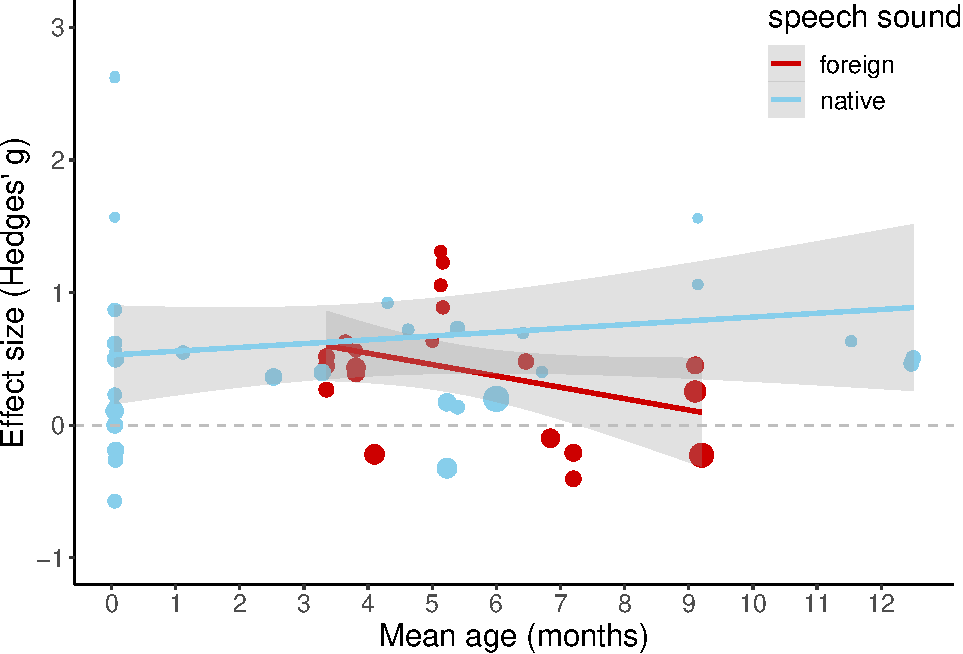
\includegraphics{MA_speech_pref_files/figure-latex/lang-1.pdf}
\caption{\label{fig:lang}Effect sizes as a function of age and familiarity with the speech sounds. The size of each dot is inversely proportional to the variance. Positive effect sizes reflect a preference for the speech sound, negative effect sizes reflect a preference for the competitor sound.}
\end{figure}

\begin{table}[tbp]

\begin{center}
\begin{threeparttable}

\caption{\label{tab:TableLang}Statistical results of meta-regression with language of the speech sounds and interaction with age. The intercept corresponds to the effect size when speech is in a foreign language at age 0. The moderator estimates correspond to changes in the intercept when the target stimuli are in the native language (familiarity).}

\begin{tabular}{lcccc}
\toprule
 & estimate & SE & t & confidence interval\\
\midrule
intercept & 0.67 & 0.29 & 2.33 & 0 - 1.34\\
familiarity & -0.42 & 0.31 & -1.37 & -1.1 - 0.26\\
familiarity * age & 0.00 & 0.00 & 2.01 & 0 - 0.01\\
\bottomrule
\end{tabular}

\end{threeparttable}
\end{center}

\end{table}

\begin{figure}
\centering
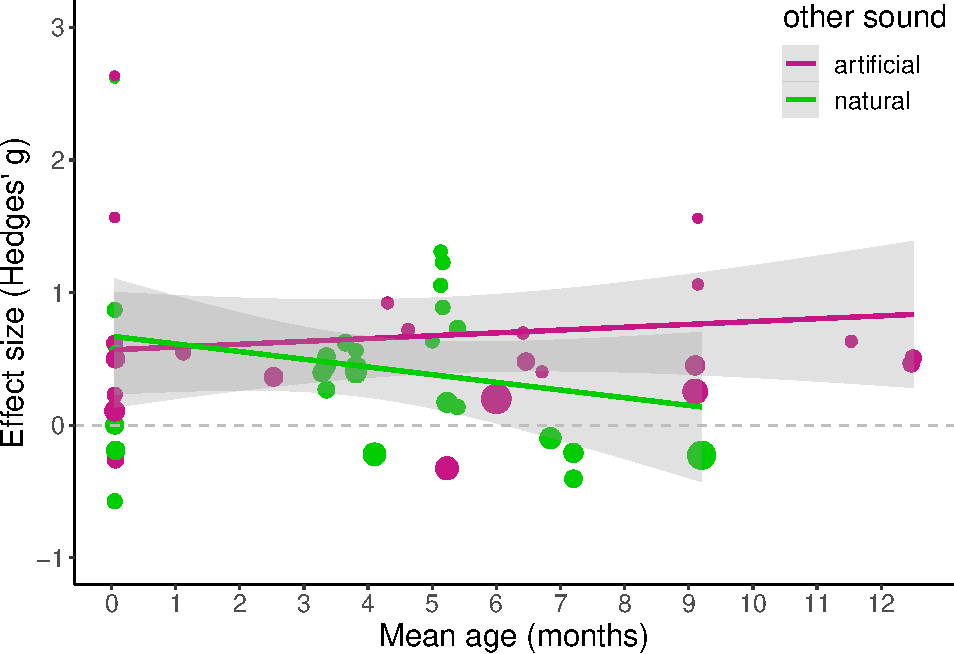
\includegraphics{MA_speech_pref_files/figure-latex/natural-1.pdf}
\caption{\label{fig:natural}Effect sizes as a function of age and natural quality of the competitor. The size of each dot is inversely proportional to the variance. Positive effect sizes reflect a preference for the speech sound, negative effect sizes reflect a preference for the competitor sound.}
\end{figure}

\begin{table}[tbp]

\begin{center}
\begin{threeparttable}

\caption{\label{tab:TableNatural}Statistical results of meta-regression with naturalness and its interaction with age as moderators. The intercept corresponds to the effect size when the competitor is natural, at age 0. The moderator estimates correspond to changes in the intercept when the competitor is artificial (naturalness).}

\begin{tabular}{lcccc}
\toprule
 & estimate & SE & t & confidence interval\\
\midrule
intercept & 0.33 & 0.22 & 1.50 & -0.21 - 0.87\\
naturalness & 0.05 & 0.24 & 0.19 & -0.47 - 0.57\\
naturalness*age & 0.00 & 0.00 & 0.71 & 0 - 0\\
\bottomrule
\end{tabular}

\end{threeparttable}
\end{center}

\end{table}

\begin{figure}
\centering
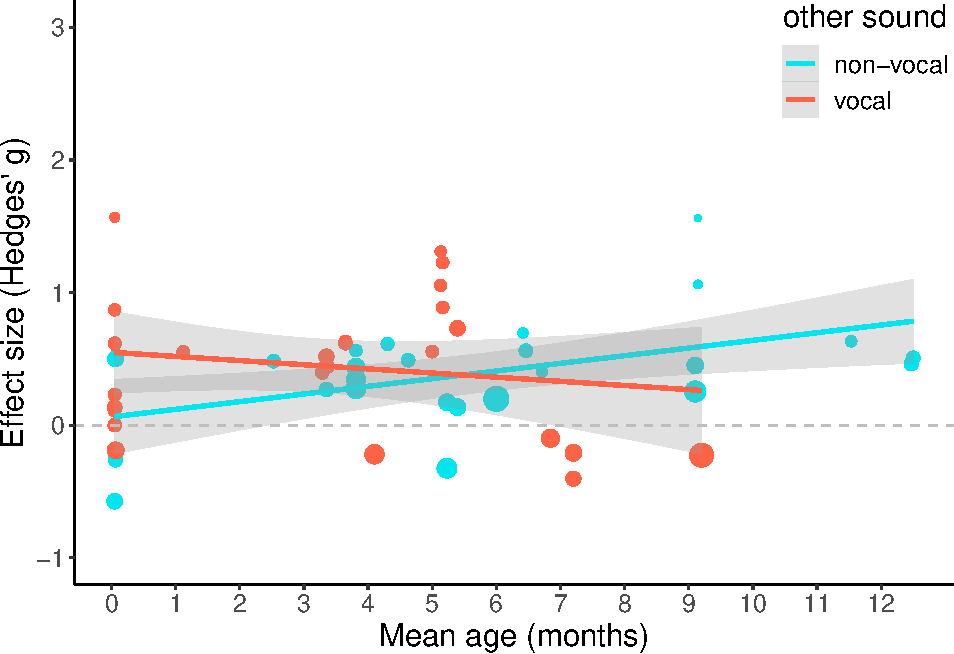
\includegraphics{MA_speech_pref_files/figure-latex/vocal-1.pdf}
\caption{\label{fig:vocal}Effect sizes as a function of age and vocal quality of the competitor. The size of each dot is inversely proportional to the variance. Positive effect sizes reflect a preference for the speech sound, negative effect sizes reflect a preference for the competitor sound.}
\end{figure}

\begin{table}[tbp]

\begin{center}
\begin{threeparttable}

\caption{\label{tab:TableVocal}Statistical results of meta-regression with vocal quality and its interaction with age as moderators. The intercept corresponds to the effect size when the competitor is vocal, at age 0. The moderator estimates correspond to changes in the intercept when the competitor is non-vocal (vocal quality).}

\begin{tabular}{lcccc}
\toprule
 & estimate & SE & t & confidence interval\\
\midrule
intercept & 0.47 & 0.16 & 2.94 & 0.1 - 0.84\\
vocal quality & -0.35 & 0.20 & -1.72 & -0.77 - 0.08\\
vocal quality*age & 0.00 & 0.00 & 2.22 & 0 - 0.01\\
\bottomrule
\end{tabular}

\end{threeparttable}
\end{center}

\end{table}

\hypertarget{discussion}{%
\section{Discussion}\label{discussion}}

Our meta-analysis synthesizes the available literature on infants' preference for speech sounds. When all experiments were considered together with no moderators, we found a sizable intercept (g=0.35, g=0.22 when taking the publication bias into account), which was still significant after correcting for the publication bias. Our meta-analysis shows that this preferential processing of speech sounds is observable from birth on. We had hypothesized age to play a major role, because it may correlate with a reshaping of the category definition for speech itself. Indeed, experiments comparing processing of human speech against human non-speech as well as animal vocalizations more generally (McDonald et al., 2019; Vouloumanos et al., 2010) often discuss these age-related differences in categorization of these sounds. Surprisingly, age did not significantly moderate the overall preference for speech, as shown by the null estimate of this moderator (Table \ref{tab:Table2}), nor did it interacted with any other moderators (Table \ref{tab:TableLang}, \ref{tab:TableNatural}, and \ref{tab:TableVocal}). This result was replicated in a separate model for age only, which showed a significant intercept, similar to the intercept found in the meta-regression with no moderator (Supplementary results S1). Crucially, age was not centered. This intercept therefore provides an estimate of the effect size at age 0, i.e.~at birth. Moreover, the scatterplot of effect sizes as a function of age reveals clearly no change with age even when plotted without other moderators (Supplementary figure S6). This null effect of age, combined with the sizable intercept, confirms that infants reliably prefer speech over other types of sounds from birth.

The significant heterogeneity we found among the literature suggests that underlying factors modulate this effect. We had predicted infants' speech preference to be larger when the competitor was an artificial sound than when it was a natural one; when the competitor was non-vocal; and when the speech was in the infants' native language. In fact, we were unable to disprove the null hypothesis of no difference for all three factors. Our meta-analysis revealed uneven distributions of experiments across age and stimulus dimensions, and that the distribution of effect sizes in the literature is consistent with publication bias. It is possible that the effect of our three moderators would emerge if the publication biased was solved. However, by aggregating the numerous individual studies of a literature, meta-analyses gain statistical power. As such, meta-analytic results have more cumulative explanatory value than single studies. Moreover, distributions of effect sizes for experiments varying along the three dimensions widely overlap. Our findings therefore suggest that none of these parameters fully explain infants' preference for speech sounds. Our dataset can be community-augmented, and we invite researchers investigating this phenomenon to complement it with any data they would have (\url{https://osf.io/4stz9/?view_only=d0696591ebf34bfc8430f848cd945ca8}), whatever the results and publication status, to solve the publication bias and confirm our findings.
This clearly points to the value of meta-analysis: to take stock of a field and inspire follow-up studies. In particular, future experiments should test infants older than 9 months. Language production gains in complexity at about this age (Oller, Eilers, Neal, \& Schwartz, 1999), which could affect infants' speech preference. Experiments using natural vocal stimuli as competitor, and foreign speech as target, would contribute to fill in the gap in the litterature that our meta-analysis revealed.

Our results suggest that, from birth on, infants show a preference for speech, which cannot be accounted by the three explanations tested here: naturalness, vocalness, or familiarity with the native language. It is possible that infants prefer speech because of its complex acoustic structure and fast transitions (Rosen \& Iverson, 2007). Spectral or temporal modulations taken separately are not sufficient to elicit neural responses similar to the ones elicited by speech (Minagawa-Kawai, Cristià, Vendelin, Cabrol, \& Dupoux, 2011). However, speech is characterized by joint spectrotemporal modulations at specific rates (Singh \& Theunissen, 2003). It is possible that infants are sensitive to this specific spectro-temporal structure (though see Norman-Haignere \& McDermott, 2018 showing that they only explain neural responses in primary auditory cortex, suggesting that other factors contribute to the behavioral response in later processing stages). Testing this explanation would require to compute the modulation spectra of the actual stimuli used in the experiments. Thus, we recommend interested researchers to deposit their stimuli in a public archive such as the Open Science Framework (Foster \& Deardorff, 2017).

A capacity to preferentially listen to speech sounds from birth suggests that infants are born with the capacity to recognize their conspecifics' communication signals. This parallels what has been proposed for faces: Infants are born with the capacity to orient their attention toward them, even without any prior exposure to faces (Morton \& Johnson, 1991; Turati, 2004). This would stem from basic perceptual abilities present at birth, namely that the visual system would be tuned to a spatial structure that correspond to those of faces (Morton \& Johnson, 1991; Turati, 2004). As newborns have never been exposed to such visual stimuli before, it would reflect general properties (i.e.~filters) of the visual system. Similarly, the auditory system could be tuned to a spectro-temporal structure that speech presents. The combination of this non-specific bias with the systematic variations of the auditory environment would result in preferential responses to speech from birth. However, contrary to faces, fetuses are exposed to speech that is low-pass filtered by the womb throughout the last trimester of gestation (Lecanuet \& Granier-Deferre, 1993; Querleu, Renard, Versyp, Paris-Delrue, \& Crèpin, 1988). It is therefore possible that prenatal experience with low-pass filtered speech helps infants to form a representation of speech, by refining the response properties of the auditory system to speech.
The fact that familiarity with the language used in the experiment did not modulate infants' preference suggests that this effect is not triggered by familiarity with the sounds of the native language. Infants would therefore form a representation that is specific enough to discriminate speech from other natural or vocal sounds, but general enough to be independant of the language spoken.

The human species is a gregarious one. Detecting speech signals allows to integrate it with other sensory percepts, such as faces, to form multisensory representations of conspecifics. Five-months old infants were capable to match human faces to speech, as well as monkey faces to monkey vocalizations (Vouloumanos et al., 2009). This provides evidence that human infants make correspondences between faces and vocalizations, and that they distinguish their conspecifics from other species. This lays the groundwork for social cognition. Finally, the preference itself may also be a meaningful index of processing that can be used to identify children at risk (Sorcinelli et al., 2019). Understanding this phenomenon is therefore crucial for both theoretical and clinical advances.

Ultimately, preferential processing of speech may support higher level cognitive tasks. Identifying speech signals and paying attention to them would allow infants to form complex representations of the sensory world, that they can manipulate cognitively. Consistently, infants could categorize visual stimuli (i.e., associate a label to a category of objects) when they were associated to speech, but not pure tones or backward speech (Ferry, Hespos, \& Waxman, 2010, 2013; Fulkerson \& Waxman, 2007). Interestingly, infants categorized visual stimuli when presented with speech, melodies, monkey (Fulkerson \& Haaf, 2003), or lemur vocalizations (Ferry et al., 2013). These results support the idea that infants' cognition is setup to respond to, and manipulate complex sounds (i.e.~modulated in time and frequency), especially those of critical ecological importance such as communicative vocalizations.

Current theories state that well before they produce their own vocal output, infants build increasingly specific speech perception abilities. Specifically, one theory argues that language develops from familiarity with the sound patterns of the language to which infants are exposed (Mehler et al., 1988). Another argues that the auditory system has evolved to process natural sounds the most efficiently (Simoncelli \& Olshausen, 2001), in which case speech would initially not be distinguished from other natural sounds. A last one argues that infants are endowed with a capacity to process vocal sounds from various species as a broad category, and narrow it to speech during the first year of life (Vouloumanos et al., 2010). With a sample size of 775 infants, covering a much wider age range than individual experiments, our meta-analysis provides evidence for yet another theoretical perspective, namely that human cognition is set up to pay attention to communication signals from conspecifics, paralleling infants' attention to faces from birth (Morton \& Johnson, 1991; Turati, 2004). Such systems may be the precursors of humans' advanced social cognition skills.

\newpage

\hypertarget{references}{%
\section{References}\label{references}}

\begingroup
\setlength{\parindent}{-0.5in}
\setlength{\leftskip}{0.5in}

\hypertarget{refs}{}
\leavevmode\hypertarget{ref-bergmann_development_2016}{}%
Bergmann, C., \& Cristia, A. (2016). Development of infants' segmentation of words from native speech: A meta-analytic approach. \emph{Developmental Science}, \emph{19}(6), 901--917. \url{https://doi.org/10.1111/desc.12341}

\leavevmode\hypertarget{ref-bergmann_promoting_2018}{}%
Bergmann, C., Tsuji, S., Piccinini, P. E., Lewis, M. L., Braginsky, M., Frank, M. C., \& Cristia, A. (2018). Promoting Replicability in Developmental Research Through Meta-analyses: Insights From Language Acquisition Research. \emph{Child Development}, \emph{89}(6), 1996--2009. \url{https://doi.org/10.1111/cdev.13079}

\leavevmode\hypertarget{ref-black_quantifying_2017}{}%
Black, A., \& Bergmann, C. (2017). Quantifying infants' statistical word segmentation: A meta-analysis. In (pp. 124--129). Cognitive Science Society. Retrieved from \url{https://pure.mpg.de/pubman/faces/ViewItemOverviewPage.jsp?itemId=item_2475527}

\leavevmode\hypertarget{ref-borenstein_introduction_2011}{}%
Borenstein, M., Hedges, L. V., Higgins, J. P. T., \& Rothstein, H. R. (2011). \emph{Introduction to Meta-Analysis}. John Wiley \& Sons.

\leavevmode\hypertarget{ref-colombo_method_1981}{}%
Colombo, J., \& Bundy, R. S. (1981). A method for the measurement of infant auditory selectivity. \emph{Infant Behavior and Development}, \emph{4}, 219--223. \url{https://doi.org/10.1016/S0163-6383(81)80025-2}

\leavevmode\hypertarget{ref-cooper_developmental_1994}{}%
Cooper, R. P., \& Aslin, R. N. (1994). Developmental Differences in Infant Attention to the Spectral Properties of Infant-Directed Speech. \emph{Child Development}, \emph{65}(6), 1663--1677. \url{https://doi.org/10.2307/1131286}

\leavevmode\hypertarget{ref-curtin_speech_2013}{}%
Curtin, S., \& Vouloumanos, A. (2013). Speech Preference is Associated with Autistic-Like Behavior in 18-Months-Olds at Risk for Autism Spectrum Disorder. \emph{Journal of Autism and Developmental Disorders}, \emph{43}(9), 2114--2120. \url{https://doi.org/10.1007/s10803-013-1759-1}

\leavevmode\hypertarget{ref-dunlap_meta-analysis_1996}{}%
Dunlap, W. P., Cortina, J. M., Vaslow, J. B., \& Burke, M. J. (1996). Meta-analysis of experiments with matched groups or repeated measures designs. \emph{Psychological Methods}, \emph{1}(2), 170--177. \url{https://doi.org/10.1037/1082-989X.1.2.170}

\leavevmode\hypertarget{ref-duval_trim_2000}{}%
Duval, S., \& Tweedie, R. (2000). Trim and Fill: A Simple Funnel-Plot--Based Method of Testing and Adjusting for Publication Bias in Meta-Analysis. \emph{Biometrics}, \emph{56}(2), 455--463. \url{https://doi.org/10.1111/j.0006-341X.2000.00455.x}

\leavevmode\hypertarget{ref-ecklund-flores_asymmetric_1996}{}%
Ecklund-Flores, L., \& Turkewitz, G. (1996). Asymmetric headturning to speech and nonspeech in human newborns. \emph{Developmental Psychobiology}, \emph{29}(3), 205--217. \href{https://doi.org/10.1002/(SICI)1098-2302(199604)29:3\%3C205::AID-DEV2\%3E3.0.CO;2-V}{https://doi.org/10.1002/(SICI)1098-2302(199604)29:3\textless{}205::AID-DEV2\textgreater{}3.0.CO;2-V}

\leavevmode\hypertarget{ref-ference_role_2018}{}%
Ference, J. D. (2018). The Role of Attentional Biases for Conspecific Vocalizations. \url{https://doi.org/http://dx.doi.org/10.11575/PRISM/31878}

\leavevmode\hypertarget{ref-ferry_categorization_2010}{}%
Ferry, A. L., Hespos, S. J., \& Waxman, S. R. (2010). Categorization in 3- and 4-Month-Old Infants: An Advantage of Words Over Tones. \emph{Child Development}, \emph{81}(2), 472--479. \url{https://doi.org/10.1111/j.1467-8624.2009.01408.x}

\leavevmode\hypertarget{ref-ferry_nonhuman_2013}{}%
Ferry, A. L., Hespos, S. J., \& Waxman, S. R. (2013). Nonhuman primate vocalizations support categorization in very young human infants. \emph{Proceedings of the National Academy of Sciences of the United States of America}, \emph{110}(38), 15231--15235. \url{https://doi.org/10.1073/pnas.1221166110}

\leavevmode\hypertarget{ref-foster_open_2017}{}%
Foster, E. D., \& Deardorff, A. (2017). Open Science Framework (OSF). \emph{Journal of the Medical Library Association : JMLA}, \emph{105}(2), 203--206. \url{https://doi.org/10.5195/jmla.2017.88}

\leavevmode\hypertarget{ref-fulkerson_influence_2003}{}%
Fulkerson, A. L., \& Haaf, R. A. (2003). The Influence of Labels, Non-Labeling Sounds, and Source of Auditory Input on 9- and 15-Month-Olds' Object Categorization. \emph{Infancy}, \emph{4}(3), 349--369. \url{https://doi.org/10.1207/S15327078IN0403_03}

\leavevmode\hypertarget{ref-fulkerson_words_2007}{}%
Fulkerson, A. L., \& Waxman, S. R. (2007). Words (but not Tones) facilitate object categorization: Evidence from 6- and 12-month-olds. \emph{Cognition}, \emph{105}(1), 218--228. \url{https://doi.org/10.1016/j.cognition.2006.09.005}

\leavevmode\hypertarget{ref-gelman_difference_2006}{}%
Gelman, A., \& Stern, H. (2006). The Difference Between ``Significant'' and ``Not Significant'' is not Itself Statistically Significant. \emph{The American Statistician}, \emph{60}(4), 328--331. \url{https://doi.org/10.1198/000313006X152649}

\leavevmode\hypertarget{ref-hedges_robust_2010}{}%
Hedges, L. V., Tipton, E., \& Johnson, M. C. (2010). Robust variance estimation in meta-regression with dependent effect size estimates. \emph{Research Synthesis Methods}, \emph{1}(1), 39--65. \url{https://doi.org/10.1002/jrsm.5}

\leavevmode\hypertarget{ref-hunter_multifactor_1988}{}%
Hunter, M. A., \& Ames, E. W. (1988). A multifactor model of infant preferences for novel and familiar stimuli. \emph{Advances in Infancy Research}, \emph{5}, 69--95.

\leavevmode\hypertarget{ref-lecanuet_speech_1993}{}%
Lecanuet, J.-P., \& Granier-Deferre, C. (1993). Speech Stimuli in the Fetal Environment. In B. de Boysson-Bardies, S. de Schonen, P. Jusczyk, P. McNeilage, \& J. Morton (Eds.), \emph{Developmental Neurocognition: Speech and Face Processing in the First Year of Life} (pp. 237--248). Dordrecht: Springer Netherlands. \url{https://doi.org/10.1007/978-94-015-8234-6_20}

\leavevmode\hypertarget{ref-lipsey_practical_2001}{}%
Lipsey, M. W., \& Wilson, D. B. (2001). \emph{Practical meta-analysis}. Thousand Oaks, CA, US: Sage Publications, Inc.

\leavevmode\hypertarget{ref-mcdonald_infant_2019}{}%
McDonald, N. M., Perdue, K. L., Eilbott, J., Loyal, J., Shic, F., \& Pelphrey, K. A. (2019). Infant brain responses to social sounds: A longitudinal functional near-infrared spectroscopy study. \emph{Developmental Cognitive Neuroscience}, \emph{36}, 100638. \url{https://doi.org/10.1016/j.dcn.2019.100638}

\leavevmode\hypertarget{ref-mehler_precursor_1988}{}%
Mehler, J., Jusczyk, P., Lambertz, G., Halsted, N., Bertoncini, J., \& Amiel-Tison, C. (1988). A precursor of language acquisition in young infants. \emph{Cognition}, \emph{29}(2), 143--178. \url{https://doi.org/10.1016/0010-0277(88)90035-2}

\leavevmode\hypertarget{ref-minagawa-kawai_assessing_2011}{}%
Minagawa-Kawai, Y., Cristià, A., Vendelin, I., Cabrol, D., \& Dupoux, E. (2011). Assessing Signal-Driven Mechanisms in Neonates: Brain Responses to Temporally and Spectrally Different Sounds. \emph{Frontiers in Psychology}, \emph{2}. \url{https://doi.org/10.3389/fpsyg.2011.00135}

\leavevmode\hypertarget{ref-mizrahi_single_2014}{}%
Mizrahi, A., Shalev, A., \& Nelken, I. (2014). Single neuron and population coding of natural sounds in auditory cortex. \emph{Current Opinion in Neurobiology}, \emph{24}, 103--110. \url{https://doi.org/10.1016/j.conb.2013.09.007}

\leavevmode\hypertarget{ref-moher_preferred_2009}{}%
Moher, D., Liberati, A., Tetzlaff, J., Altman, D. G., \& Group, T. P. (2009). Preferred Reporting Items for Systematic Reviews and Meta-Analyses: The PRISMA Statement. \emph{PLOS Medicine}, \emph{6}(7), e1000097. \url{https://doi.org/10.1371/journal.pmed.1000097}

\leavevmode\hypertarget{ref-moon_two-day-olds_1993}{}%
Moon, C., Cooper, R. P., \& Fifer, W. P. (1993). Two-day-olds prefer their native language. \emph{Infant Behavior and Development}, \emph{16}(4), 495--500. \url{https://doi.org/10.1016/0163-6383(93)80007-U}

\leavevmode\hypertarget{ref-morton_conspec_1991}{}%
Morton, J., \& Johnson, M. H. (1991). CONSPEC and CONLERN: A Two-Process Theory of Infant Face Recognition. \emph{Psychological Review}, \emph{98}(2), 164--181.

\leavevmode\hypertarget{ref-norman-haignere_neural_2018}{}%
Norman-Haignere, S. V., \& McDermott, J. H. (2018). Neural responses to natural and model-matched stimuli reveal distinct computations in primary and nonprimary auditory cortex. \emph{PLOS Biology}, \emph{16}(12), e2005127. \url{https://doi.org/10.1371/journal.pbio.2005127}

\leavevmode\hypertarget{ref-oakes_sample_2017}{}%
Oakes, L. M. (2017). Sample Size, Statistical Power, and False Conclusions in Infant Looking-Time Research. \emph{Infancy}, \emph{22}(4), 436--469. \url{https://doi.org/10.1111/infa.12186}

\leavevmode\hypertarget{ref-oller_precursors_1999}{}%
Oller, D. K., Eilers, R. E., Neal, A. R., \& Schwartz, H. K. (1999). Precursors to speech in infancy: The prediction of speech and language disorders. \emph{Journal of Communication Disorders}, \emph{32}(4), 223--245. \url{https://doi.org/10.1016/S0021-9924(99)00013-1}

\leavevmode\hypertarget{ref-poremba_processing_2013}{}%
Poremba, A., Bigelow, J., \& Rossi, B. (2013). Processing of communication sounds: Contributions of learning, memory, and experience. \emph{Hearing Research}, \emph{305}, 31--44. \url{https://doi.org/10.1016/j.heares.2013.06.005}

\leavevmode\hypertarget{ref-querleu_fetal_1988}{}%
Querleu, D., Renard, X., Versyp, F., Paris-Delrue, L., \& Crèpin, G. (1988). Fetal hearing. \emph{European Journal of Obstetrics \& Gynecology and Reproductive Biology}, \emph{28}(3), 191--212. \url{https://doi.org/10.1016/0028-2243(88)90030-5}

\leavevmode\hypertarget{ref-r_core_team_r:_2018}{}%
R Core Team. (2018). R: A Language and Environment for Statistical Computing. Vienna, Austria: R Foundation for Statistical Computing. Retrieved from \url{https://www.R-project.org}

\leavevmode\hypertarget{ref-rosen_constructing_2007}{}%
Rosen, S., \& Iverson, P. (2007). Constructing adequate non-speech analogues: What is special about speech anyway? \emph{Developmental Science}, \emph{10}(2), 165--168. \url{https://doi.org/10.1111/j.1467-7687.2007.00550.x}

\leavevmode\hypertarget{ref-santolin_role_2019}{}%
Santolin, C., Russo, S., Calignano, G., Saffran, J. R., \& Valenza, E. (2019). The role of prosody in infants' preference for speech: A comparison between speech and birdsong. \emph{Infancy}, \emph{24}(5), 827--833. \url{https://doi.org/10.1111/infa.12295}

\leavevmode\hypertarget{ref-santolin_infants_2020}{}%
Santolin, C., Zettersten, M., \& Saffran, J. R. (2020). Infants' preference for non-native speech versus birdsong. Unpublished data. Retrieved from \url{https://github.com/mzettersten/birdsong}

\leavevmode\hypertarget{ref-segal_listening_2011}{}%
Segal, O., \& Kishon-Rabin, L. (2011). Listening Preference for Child-Directed Speech Versus Nonspeech Stimuli in Normal-Hearing and Hearing-Impaired Infants After Cochlear Implantation Ovid. \emph{Ear and Hearing}, \emph{32}(3), 358--372. \url{https://doi.org/10.1097/AUD.0b013e3182008afc}

\leavevmode\hypertarget{ref-shultz_three-month-olds_2010}{}%
Shultz, S., \& Vouloumanos, A. (2010). Three-Month-Olds Prefer Speech to Other Naturally Occurring Signals. \emph{Language Learning and Development}, \emph{6}(4), 241--257. \url{https://doi.org/10.1080/15475440903507830}

\leavevmode\hypertarget{ref-simoncelli_natural_2001}{}%
Simoncelli, E. P., \& Olshausen, B. A. (2001). Natural image statistics and neural representation. \emph{Annual Review of Neuroscience}, \emph{24}, 1193--1216. \url{https://doi.org/10.1146/annurev.neuro.24.1.1193}

\leavevmode\hypertarget{ref-singh_modulation_2003}{}%
Singh, N. C., \& Theunissen, F. E. (2003). Modulation spectra of natural sounds and ethological theories of auditory processing. \emph{The Journal of the Acoustical Society of America}, \emph{114}(6), 3394. \url{https://doi.org/10.1121/1.1624067}

\leavevmode\hypertarget{ref-smith_efficient_2006}{}%
Smith, E. C., \& Lewicki, M. S. (2006). Efficient auditory coding. \emph{Nature}, \emph{439}(7079), 978--982. \url{https://doi.org/10.1038/nature04485}

\leavevmode\hypertarget{ref-sorcinelli_preference_2019}{}%
Sorcinelli, A., Ference, J., Curtin, S., \& Vouloumanos, A. (2019). Preference for speech in infancy differentially predicts language skills and autism-like behaviors. \emph{Journal of Experimental Child Psychology}, \emph{178}, 295--316. \url{https://doi.org/10.1016/j.jecp.2018.09.011}

\leavevmode\hypertarget{ref-spence_prenatal_1987}{}%
Spence, M. J., \& DeCasper, A. J. (1987). Prenatal experience with low-frequency maternal-voice sounds influence neonatal perception of maternal voice samples. \emph{Infant Behavior and Development}, \emph{10}(2), 133--142. \url{https://doi.org/10.1016/0163-6383(87)90028-2}

\leavevmode\hypertarget{ref-turati_why_2004}{}%
Turati, C. (2004). Why Faces Are Not Special to Newborns: An Alternative Account of the Face Preference. \emph{Current Directions in Psychological Science}, \emph{13}(1), 5--8. \url{https://doi.org/10.1111/j.0963-7214.2004.01301002.x}

\leavevmode\hypertarget{ref-vanden_bosch_der_nederlanden_infant_2020}{}%
Vanden Bosch der Nederlanden, C. M., \& Vouloumanos, A. (2020). Infant biases for detecting speech in complex scenes. \emph{Under Review}.

\leavevmode\hypertarget{ref-vouloumanos_foundational_2014}{}%
Vouloumanos, A., \& Curtin, S. (2014). Foundational Tuning: How Infants' Attention to Speech Predicts Language Development. \emph{Cognitive Science}, \emph{38}(8), 1675--1686. \url{https://doi.org/10.1111/cogs.12128}

\leavevmode\hypertarget{ref-vouloumanos_five-month-old_2009}{}%
Vouloumanos, A., Druhen, M. J., Hauser, M. D., \& Huizink, A. T. (2009). Five-month-old infants' identification of the sources of vocalizations. \emph{Proceedings of the National Academy of Sciences of the United States of America}, \emph{106}(44), 18867--18872. \url{https://doi.org/10.1073/pnas.0906049106}

\leavevmode\hypertarget{ref-vouloumanos_tuning_2010}{}%
Vouloumanos, A., Hauser, M. D., Werker, J. F., \& Martin, A. (2010). The tuning of human neonates' preference for speech. \emph{Child Development}, \emph{81}(2), 517--527. \url{https://doi.org/10.1111/j.1467-8624.2009.01412.x}

\leavevmode\hypertarget{ref-vouloumanos_tuned_2004}{}%
Vouloumanos, A., \& Werker, J. F. (2004). Tuned to the signal: The privileged status of speech for young infants. \emph{Developmental Science}, \emph{7}(3), 270--276. \url{https://doi.org/10.1111/j.1467-7687.2004.00345.x}

\leavevmode\hypertarget{ref-vouloumanos_listening_2007}{}%
Vouloumanos, A., \& Werker, J. F. (2007). Listening to language at birth: Evidence for a bias for speech in neonates. \emph{Developmental Science}, \emph{10}(2), 159--164. \url{https://doi.org/10.1111/j.1467-7687.2007.00549.x}

\leavevmode\hypertarget{ref-yamashiro_does_2019}{}%
Yamashiro, A., Curtin, S., \& Vouloumanos, A. (2019). Does an Early Speech Preference Predict Linguistic and Social-Pragmatic Attention in Infants Displaying and Not Displaying Later ASD Symptoms? \emph{Journal of Autism and Developmental Disorders}. \url{https://doi.org/10.1007/s10803-019-03924-2}

\endgroup

\end{document}
